\documentclass[fontsize=12pt,paper=a4,twoside]{scrartcl}
\usepackage{longtable} 
\usepackage{graphicx}
% SWP-Präambel
% C 2003-2017 Sebastian Offermann, Rainer Koschke, Karsten Hölscher
% In Zeilen 40 und 41 sind jeweils die aktuellen Daten einzutragen

\usepackage[utf8]{inputenc}     % Kodierung der Tex-Datei
\usepackage[T1]{fontenc}        % Korrekte Ausgabe von Sonderzeichen (Umlaute)
\usepackage[ngerman]{babel}     % Deutsche Einstellungen [ab \begin{document}]

\usepackage{bibgerm}            % Bibliographie
\usepackage{fancyhdr}           % obere Seitenränder gestalten
\usepackage{float}              % Floats Objekte mit [H] festsetzen
\usepackage{graphicx}           % Graphiken als jpg, png etc. einbinden
\usepackage{moreverb}           % zusätzliche verbatim-Umgebungen
\usepackage{pdflscape}          % PDF-Support für landscape
\usepackage[final]{pdfpages}    % Externe PDFs einbinden
\usepackage{stmaryrd}           % zusätzliche Symbole
\usepackage{supertabular}       % Tabellen über Seitenränder hinaus
\usepackage{tabularx}           % Tabellen mit vorgegebener Breite
\usepackage{url}                % setzt URLs schön mit \url{http://bla.laber.com/~mypage}

%%% Die Reihenfolge der folgenden Pakete muss beibehalten werden:
%%% varioref, hyperref, cleveref, bookmark
% Verweise innerhalb des Dokuments schick mit " ... auf Seite ... "
% automatisch versehen. Dazu \vref{labelname} benutzen
\usepackage[ngerman]{varioref}  % [vor hyperref für korrekte Verweise]
\usepackage[colorlinks=true, pdfstartview=FitV, linkcolor=blue,
            citecolor=blue, urlcolor=blue, hyperfigures=true,
            pdftex=true]{hyperref} % [vor bookmark wegen der Optionen]
\usepackage[ngerman]{cleveref}
\usepackage{bookmark}

\hyphenation{Arbeits-paket}     % Trennungsregeln

%%% Definitionen
\newcommand{\grad}{\ensuremath{^{\circ}} }
\renewcommand{\strut}{\vrule width 0pt height5mm depth2mm}
\newcommand{\gq}[1]{\glqq{}#1\grqq{}}

%%% Semesterkonstanten
\newboolean{langversion} %Deklaration
\setboolean{langversion}{true} %Zuweisung ist 'false' für Blockkurs
\newcommand{\jahr}[1]{2020} %2017/2018

% erstes Argument: SWP-2, zweites SWP-1
\newcommand{\highlight}[1]{\textcolor{blue}{\textbf{#1}}}
\newcommand{\variante}[2]{\ifthenelse{\boolean{langversion}}{#1}{#2}}
\newcommand{\nurlangversion}[0]%
    {\variante{\highlight{}}%Muss in SWP-2 ausgefüllt werden}}%
              {\highlight{Entfällt in SWP-1}}}
\newcommand{\swp}[0]{Software-Projekt \variante{2}{1}}
\newcommand{\semester}[0]{SoSe \jahr}

%%% Formatierungsanpassungen
% Damit Latex nicht zu lange Zeilen produziert:
\sloppy
%Uneinheitlicher unterer Seitenrand:
%\raggedbottom

% Kein Erstzeileneinzug beim Absatzanfang
% Sieht aber nur gut aus, wenn man zwischen Absätzen viel Platz einbaut
\setlength{\parindent}{0ex}

% Abstand zwischen zwei Absätzen
\setlength{\parskip}{1ex}

% Seitenränder für Korrekturen verändern
\addtolength{\evensidemargin}{-1cm}
\addtolength{\oddsidemargin}{1cm}

\bibliographystyle{gerapali}

% 1. Parameter: Euer/Eure TutorIn, z. B. {Kim Harrison}
% 2. Parameter: Abgabedatum, z. B. {05. April 2063}
% 3. Parameter: Versionsnummer, z. B. {1.1}
% 4.-9. Parameter: jeweils Name und (Uni-)Email-Adresse jedes 
%                 Gruppenmitglieds; mit einem & getrennt, z. B.
% {Robin Cowl & roco@tzi.de}
% Besteht die Gruppe aus weniger als 6 Personen, so werden die 
% übrigen Parameter leer gelassen: {}
\newcommand \swpdocument[9] {
% Lustige Header auf den Seiten
  \pagestyle{fancy}
  \setlength{\headheight}{70.55003pt}
  \fancyhead{}
  \fancyhead[LO,RE]{\swp{}\\%
                    \semester{}\\%
                    \documentTitle}
  \fancyhead[LE,RO]{Seite \thepage\\%
                    \slshape \leftmark\\%
                    \slshape \rightmark}

% Lustige Header nur auf dieser Seite (Titelseite)
  \thispagestyle{fancy}
  \fancyhead[LO,RE]{ }
  \fancyhead[LE,RO]{Universität Bremen\\%
                    FB 3 -- Informatik\\%
                    Dr. Karsten Hölscher\\%
                    TutorIn: #1}
  \fancyfoot[C]{}

% Start Titelseite
  \vspace{3cm}
  \begin{minipage}[H]{\textwidth}
    \begin{center}
      \bfseries \Large \swp{} -- \semester{}\\
      \smallskip
      \small VAK 03-BA-901.02\\
      \vspace{3cm}
    \end{center}
  \end{minipage}
  \begin{minipage}[H]{\textwidth}
    \begin{center}
      \vspace{1cm}
      \bfseries \Large \documentTitle\\
      \vfill
    \end{center}
  \end{minipage}
  \vfill
  \begin{minipage}[H]{\textwidth}
    \begin{center}
      \sffamily
      \begin{tabular}{lr}
        #4 \\
        #5 \\
        #6 \\
        #7 \\
        #8 \\
        #9 \\
      \end{tabular}
      \\[22mm]
      \itshape Abgabe: #2 --- Version #3 \\ ~
    \end{center}
  \end{minipage}
% Ende Titelseite

% Start Inhaltsverzeichnis
\newpage
  \thispagestyle{fancy}
  \fancyhead{}
  \fancyhead[LO,RE]{\swp{}\\%
                    \semester{}\\%
                    \documentTitle}
  \fancyhead[LE,RO]{Seite \thepage\\%
                    \slshape \leftmark\\~}
  \fancyfoot{}
  \renewcommand{\headrulewidth}{0.4pt}
  \tableofcontents
% Ende Inhaltsverzeichnis

% Header für alle weiteren Seiten
\newpage
  \fancyhead[LE,RO]{Seite \thepage\\%
                    \slshape \leftmark\\%
                    \slshape \rightmark}

}



%
% Und jetzt geht das Dokument los....
%
\begin{document}
\newcommand\documentTitle{Architekturbeschreibung}
\swpdocument{Euer/Eure TutorIn}{TT. Monat JJJJ}{1.1}%
            {Clara Maria Odinius & odinius@uni-bremen.de}%
            {Habib Mergan & habib1@uni-bremen.de}%
            {Kevin Santiago Rey Rodriguez & kev\_rey@uni-bremen.de}%
            {Liam Hurwitz & hurwitz@uni-bremen.de}%
            {Mehmet Ali Baykara & baykara@uni-bremen.de}%
            {Miguel Alejandro Caceres Pedraza & mcaceres@uni-bremen.de}%

%%%%%%%%%%%%%%%%%%%%%%%%%%%%%%%%%%%%%%%%%%%%%%%%%%%%%%%%%%%%%%%%%%%%%%%%
\section*{Version und Änderungsgeschichte}

{\em Die aktuelle Versionsnummer des Dokumentes sollte eindeutig und gut zu
identifizieren sein, hier und optimalerweise auf dem Titelblatt.}

\begin{tabular}{ccl}
Version & Datum & Änderungen \\
\hline
0.1 & TT.MM.JJJJ & Dokumentvorlage als initiale Fassung kopiert \\
0.2 & TT.MM.JJJJ & \ldots \\
\ldots
\end{tabular}


%%%%%%%%%%%%%%%%%%%%%%%%%%%%%%%%%%%%%%%%%%%%%%%%%%%%%%%%%%%%%%%%%%%%%%%%
\section{Einführung}

\subsection{Zweck}

{ \em Was ist der Zweck dieser Architekturbeschreibung? Wer sind die LeserInnen?}

\subsection{Status}
  
\subsection{Definitionen, Akronyme und Abkürzungen}
  \begin{longtable}{ |  l | p{12cm} |}
    \hline
    Begriff & Definition \\ \hline
Software-Architektur &Beschreibt die grundlegende Komponenten eines
Softwaresystems.\\ \hline
Architektursicht (View) &Repräsentation eines ganzen Systems
aus der Perspektive einer kohärenten Menge von
Anliegen (IEEE P1471, 2002). \\ \hline
 Anwendungsfälle & Spezifiziert eine beliebige Menge von Aktionen, die
ein System ausführen muss, damit ein Resultat stattfindet,
welches für mindestens einen Akteur von Bedeutung
ist. \\ \hline
    Framework &Programmiergerüst, welches den Rahmen der Anwendung
bildet. Es umfasst Bibliotheken und Komponenten. \\ \hline
    UML &Steht für Unified Modeling Language und ist eine grafische
Modellierungssprache zur Spezifikation, Visualisierung,
Konstruktion und Dokumentation von Modellen
für Softwaresysteme. \\
    \hline
IDE & integrierte Entwicklungsumgebung - Hilft bei der Bearbeitung von Projekten
in der Softwareentwicklung. \\     \hline
Versionskontrolle  &Hochgeladenen Versionen werden festgehalten und können
wieder hergestellt werden. \\     \hline
 Maven  &Java Programme können standardisiert und verwaltet werden.\\     \hline
 Library &Sammlung von verschiedensten vorgefertigten Methoden oder Klassen.\\     \hline
Interface &Schnittstelle.\\     \hline
Multiplayer &Spielmodus, mit mehr als einem Spieler zur gleichen Zeit.\\    \hline
Singleplayer &Spielmodus, mit einem Spieler, der gegen einen computergesteuerten
Gegner spielt. \\     \hline
JUnit & Frameworke für Tests für die Programmiersprache Java.\\     \hline
Javadoc  &Software-Dokumentationswerkzeug für die Programmiersprache Java. \\     \hline
JavaEE &(Java Platform Enterprise Edition) Eine Spezifikation für die transaktionsbasierte 
Ausführung von in Java programmierten Anwendungen.\\    \hline
GUI &Steht für Graphical User Interface und kennzeichnet
eine grafische Schnittstelle, über die ein Mensch mit
einer Software interagiert.\\ \hline
Paketdiagramm &Strukturdiagramm der UML, stellt die Verbindung
zwischen Paketen, Paketimports bzw. Verschmelzungen
und deren Abhängigkeiten dar. \\ \hline
Problemkarte &Beschreiben Probleme im Zusammengang der Einflussfaktoren
und stellen Lösungen bzw. entsprechende
Strategien dar. \\ \hline
Sequenzdiagramm &Strukturdiagramm der UML, stellt den Austausch
von Nachrichten zwischen Objekten mittels einer Lebenslinie
dar. \\ \hline
Klassendiagramm &Strukturdiagramm der UML, stellt die statischen
Strukturen eines Systems dar.\\ \hline
Komponentendiagramm &Strukturdiagramm der UML, stellt Komponenten
und deren Schnittstellen dar. \\ \hline
HTTP &Steht für Hypertext Transfer Protocol, einem zustandslosen
Protokoll zum synchronen Versenden von
Informationen über Rechnernetze.\\ \hline
HTTPS &Durch Verschlüsselungstechniken gesichertes HTTP. \\ \hline
TCP &Das Transmission Control Protocol ist ein Netzwerkprotokoll, das definiert, auf welche Art und Weise
 Daten zwischen Netzwerkkomponenten ausgetauscht werden sollen. \\ \hline
UDP &Das User Datagram Protocol, kurz UDP, ist ein minimales, verbindungsloses Netzwerkprotokoll, 
das zur Transportschicht der Internetprotokollfamilie gehört.\\ \hline
   

 \end{longtable}

\subsection{Referenzen}
Vorlesungsfolien


\subsection{Übersicht über das Dokument}

%%%%%%%%%%%%%%%%%%%%%%%%%%%%%%%%%%%%%%%%%%%%%%%%%%%%%%%%%%%%%%%%%%%%%%%%
\newpage
\section{Anwendungsfälle} \label{sec:Anwendungsfälle}
\subsection{Anmeldung}
Ein User startet das Spiel. Ein Fenster, in dem sich der  User mit Password und Namen einloggen  kann, öffnet sich. Wenn er die richtige Daten einträgt. kann das Spielt  weiter geführt werden. Falls die Daten nicht richtig sind, bekommt der User  einen Hinweis darauf und wird geben es erneut zu versuchen.
\subsection{Multi-Spieler}
Wenn der User angemeldet ist, dann kann er sehen, welche der andere User ebenfalls verbunden sind und hat entweder die Möglichkeit gegen ander User zu spielen oder aber ein Spiel gegen den Computer zu starten.
\subsection{Spielt-Starten}
Im ersten Fenster des Spiels kann der Benutzer das Raumschiff, die Waffen, welche er verwenden möchte, die Besatzung und den Schwierigkeitsgrad des Spiels auswählen. Anschließend startet das Spiel.
\subsection{Spielt-Verlauft}
Zu beginn, kann der Spieler die Crew in den von ihm gewählten Positionen/Sektionen des Raumschiffes positionieren. Dann kann er die Sprungtaste drücken, um die Zielplaneten auszuwählen. Der Benutzer kann dies  in jeder Runde wiederholen.

Wenn der Benutzer einen Zielplaneten auswählt, kann er auf Gegner treffen und nach einem Dialogfeld gegen diese antreten.

Sobald der Benutzer gewonnen hat,  kann der Gegner sein Raumschiff reparieren, seine Crew heilen oder einen Sprung machen.

\subsection{Kampf-Regeln}
In einem Kampf gelten folgende Regeln:
\begin{itemize}
\item Wenn ein Kampf beginnt, kann der Benutzer dseine Waffen ausrichten, um auf  bestimmte Sektionen des gegnerischen Raumschiffes zu zielen.
 
\item Waffen brauchen Zeit zum Laden und Schießen.

\item Damit eine Waffe das Ziel treffen kann, muss der Gegner Schilde deaktiviert haben.

\item Um die Schilde zu deaktivieren, müssen diese zuvor x mal getroffen worden sein. Je Treffer auf das Schild,  verliert es an Stärke. Sobald die Stärke des Schildes Null ist, ist es deaktiviert.

\item Waffen treffen zu bestimmten Wahrscheinlichkeiten  das Ziel.

\item Damit eine Waffe verwendet werden kann, muss die Sektion, in der die Waffe steht, funktionsfähig sein, sowie sich ein Besatzungsmitglied in selbiger Sektion aufghalten muss, damit diese auch bedient werden können.

\item Jedes Mal, wenn eine Waffe ein Raumschiff trifft, verliert sie ihren Lebenspunkt.

\item Sobald eines der beiden Raumschiffe keine Lebenspunkte mehr hat, hat es verloren.
\end{itemize}
\subsection{Pausenmodus}
Während eines Kampfes kann der Benutzer das Spiel in den Pausenmodus versetzen. Somit sind für Beide Parteien alle Spielzüge eingefrohren,  wenn das Spiel fortgesetzt wird, wird an selber Stelle fort gefahren.
\newpage
%%%%%%%%%%%%%%%%%%%%%%%%%%%%%%%%%%%%%%%%%%%%%%%%%%%%%%%%%%%%%%%%%%%%%%%%
\section{Globale Analyse} \label{sec:globale_analyse}



\subsection{Einflussfaktoren} \label{sec:einflussfaktoren}
%{\itshape Hier sind Einflussfaktoren gefragt, die sich auf die Architektur
%beziehen. Es sind ausschließlich architekturrelevante Einflussfaktoren, und 
%nicht z.\,B.\ solche, die lediglich einen Einfluss auf das Projektmanagement 
%haben. Fragt Euch also bei jedem Faktor: Beeinflusst er wirklich die 
%Architektur? Macht einen einfachen Test: Wie würde die Architektur aussehen, 
%wenn ihr den Einflussfaktor $E$ berücksichtigt? Wie würde sie aussehen, wenn Ihr
%$E$ nicht berücksichtigt? Kommt in beiden Fällen dieselbe Architektur heraus, 
%dann kann der Einflussfaktor nicht architekturrelevant sein.

%Es geht hier um Einflussfaktoren, die
%\begin{enumerate}
%  \item sich über die Zeit ändern,
%  \item viele Komponenten betreffen,
%  \item schwer zu erfüllen sind oder
%  \item mit denen man wenig Erfahrung hat.
%\end{enumerate}

%Die Flexibilität und Veränderlichkeit müssen ebenfalls charakterisiert werden. 
%\begin{enumerate}
%  \item Flexibilität: Könnt Ihr den Faktor zum jetzigen Zeitpunkt beeinflussen?
%  \item Veränderlichkeit: ändert der Faktor sich später durch äußere Einflüsse?
%\end{enumerate}

%Unter Auswirkungen sollte dann beschrieben werden, \emph{wie} der Faktor 
%\emph{was} beeinflusst. Das können sein:
%\begin{itemize}
%  \item andere Faktoren
%  \item Komponenten
%  \item Operationsmodi
%  \item Designentscheidungen (Strategien)
%\end{itemize}

%Verwendet eine eindeutige Nummerierung der Faktoren, um sie auf den 
%Problemkarten einfach referenzieren zu können.}


%%START einflussfaktoren

%\begin{table}[H]
%\centering
\begin{longtable}{|p{1cm}|p{3cm}|p{5cm}|p{1cm}|p{5cm}|}
\hline
\begin{tabular}[c]{@{}l@{}}Abge-\\ leitet\\aus\end{tabular} & Einflussfaktor                                                                        & \begin{tabular}[c]{@{}l@{}}Flexibilität und \\ Veränderlichkeit\end{tabular}                                                              & \begin{tabular}[c]{@{}l@{}}++/\\\\ - -\end{tabular} & Auswirkungen                                                                                                                                                                                                                              \\ \hline
\multicolumn{5}{|l|}{O1 : Organisation}                                                                                                                                                                                                                                                                                                                                                                                                                                                                                                                                                          \\ \hline
\multicolumn{5}{|l|}{O1.1 Time-To-Market}                                                                                                                                                                                                                                                                                                                                                                                                                                                                                                                                                        \\ \hline
													& \begin{tabular}[c]{@{}l@{}}Die Auslieferung\\  erfolgt am\\  02.08.2020.\end{tabular} & \begin{tabular}[c]{@{}l@{}}Keine\\ Veränderlichkeit oder \\Flexibilität, da \\ Vorgaben bestehen.\end{tabular} & \begin{tabular}[c]{@{}l@{}}- -/\\   - -\end{tabular} & \begin{tabular}[c]{@{}l@{}}Nicht alle\\  Funktionen können\\  realisiert werden \\ bzw. implementiert werden.\end{tabular}                                                                                                                                             \\ \hline
\multicolumn{5}{|l|}{O1.2 Architektur-Abgabe}                                                                                                                                                                                                                                                                                                                                                                                                                                                                                                                                                    \\ \hline
													& \begin{tabular}[c]{@{}l@{}}Die Auslieferung \\erfolgt am\\ 31.05.2020.\end{tabular}      & \begin{tabular}[c]{@{}l@{}}Keine\\ Veränderlichkeit oder \\Flexibilität, da \\ Vorgaben bestehen.\end{tabular} & \begin{tabular}[c]{@{}l@{}}- -/\\   - -\end{tabular} & \begin{tabular}[c]{@{}l@{}}Durch den\\ Zeitdruck könnte\\ die Architektur\\ mangelhaft\\ werden. Wenn wir\\ uns nicht genug\\ Zeit lassen,\\ könnten Aspekte,\\ die relevant für die\\ Architektur sind,\\ vergessen werden.\end{tabular} \\ \hline
\multicolumn{5}{|l|}{O1.3 Entwickler}                                                                                                                                                                                                                                                                                                                                                                                                                                                                                                                                                    \\ \hline
													& \begin{tabular}[c]{@{}l@{}}Die\\ Projektgruppe \\besteht aus\\ 6 Entwicklern\\\end{tabular}      & \begin{tabular}[c]{@{}l@{}}Falls ein Entwickler \\ (temporär) ausfällt kann\\ ein anderer Entwickler\\ einspringen. \\ Keine neuen Entwickler \\
können eingestellt \\ werden. Gruppenmitglieder\\ können wegfallen oder \\ austreten\end{tabular} & \begin{tabular}[c]{@{}l@{}}+/\\   - -\end{tabular} & \begin{tabular}[c]{@{}l@{}} Die Architektur kann \\wegen Zeitmangel (es \\können nicht mehr \\als die ursprünglichen\\ sechs Entwickler mitarbeiten) \\und fehlenden Fähigkeiten\\ Mängel enthalten. \\ Unvollständige\\ Implementierung droht \end{tabular} \\ \hline

\multicolumn{5}{|l|}{O1.4 Fähigkeiten Entwickler}                                                                                                                                                                                                                                                                                                                                                                                                                                                                                                                                                    \\ \hline
													& \begin{tabular}[c]{@{}l@{}}Nicht alle \\ Entwickler \\ haben die gleiche \\ Programmier-\\erfahrung \end{tabular}      & \begin{tabular}[c]{@{}l@{}}Hohe Veränderlichkeit\\ und Flexibilität durch \\Ausführen des Projekts und \\Recherche.\\ TODO! \end{tabular} & \begin{tabular}[c]{@{}l@{}}++/\\   ++\end{tabular} & \begin{tabular}[c]{@{}l@{}}Die Implementierung \\ kann Mängel enthalten. \\\end{tabular} \\ \hline

\newpage

\hline									
\multicolumn{5}{|l|}{O1.5 Teamarbeit in Corona-Zeiten}                                                                                                                                                                                                                                                                                                                                                                                                                                                                                                                                                    \\ \hline

& \begin{tabular}[c]{@{}l@{}}
Das persönliche\\ Treffen kann \\nicht stattfinden,\\ aufgrund von\\ Kontakt- \\beschränkung \end{tabular}      & \begin{tabular}[c]{@{}l@{}} Digitale Treffen über z.B.\\ Discord. Keine \\Veränderlichkeit\\ aufgrund der \\ Gesetzeslage. \end{tabular} & \begin{tabular}[c]{@{}l@{}}++/\\   - -\end{tabular} & \begin{tabular}[c]{@{}l@{}}Missverständnisse \\können öfter\\auftreten.\\Teamarbeit könnte\\erschwert werden\\ und dadurch\\die Qualität der\\der Architektur\\beeinträchtigen
\\\end{tabular} \\ \hline
%%\end{tabular}
\end{longtable}

%%%%%%
%%%%%%

%%\begin{table}[H]
%%\centering
\begin{longtable}{|p{1cm}|p{3cm}|p{5cm}|p{1cm}|p{5cm}|}
\hline
\begin{tabular}[c]{@{}l@{}}Abge-\\ leitet\\aus\end{tabular} & Einflussfaktor                                                                        & \begin{tabular}[c]{@{}l@{}}Flexibilität und \\ Veränderlichkeit\end{tabular}                                                              & \begin{tabular}[c]{@{}l@{}}++/\\\\ - -\end{tabular} & Auswirkungen                                                                                                                                                                                                                              \\ \hline
\multicolumn{5}{|l|}{T1: Technik}
\\ \hline
\multicolumn{5}{|l|}{T1.1: Programmiersprache}                                                                                                                                                                                                                                                                                                                                                                                                                                                                                                                                                    \\ \hline
                                                          & \begin{tabular}[c]{@{}l@{}}Java 8 \\ oder höher ist \\ vorgegeben.\end{tabular}      & \begin{tabular}[c]{@{}l@{}}Die Programmier-\\sprache wird vorgegeben.\\ Wir können aber\\zwischen verschiedenen\\Versionen auswählen.\end{tabular} & \begin{tabular}[c]{@{}l@{}}- -/\\   o\end{tabular} & \begin{tabular}[c]{@{}l@{}}Das Architektur muss\\ in Java umgesetzt \\werden.\end{tabular} \\ \hline

\multicolumn{5}{|l|}{T1.2 Betriebssystem}                                                                                                                                                                                                                                                                                                                                                                                                                                                                                                                                                    \\ \hline
                                                          & \begin{tabular}[c]{@{}l@{}}Die Anwendung \\muss auf den\\gängigen\\ Betriebssystemen\\(MacOS,\\ Windows, Linux) \\ laufen. \end{tabular}      & \begin{tabular}[c]{@{}l@{}}Keine\\ Veränderlichkeit oder \\Flexibilität, da\\ Mindestanforderungen\\ bestehen. Aber wir können\\ noch weitere\\ Betriebssysteme\\ hinzufügen\end{tabular} & \begin{tabular}[c]{@{}l@{}}- -/\\   - -\end{tabular} & \begin{tabular}[c]{@{}l@{}}Bei der Implementierung \\ müssen die gängigen\\ Betriebssysteme\\ berücksichtigt werden.\\ Wenn die Anwendung\\auf mehr\\Betriebssystemen\\laufen soll, dann\\ muss mehr Zeit\\investiert werden. \end{tabular} \\ \hline

\multicolumn{5}{|l|}{T1.3 Client-Server-Architektur TODO!}                                                                                                                                                                                                                                                                                                                                                                                                                                                                                                                                                    \\ \hline
                                                          & \begin{tabular}[c]{@{}l@{}}Zur\\ Implementierung\\ muss JavaEE 11\\ benutzt werden. \end{tabular}      & \begin{tabular}[c]{@{}l@{}}Keine\\ Veränderlichkeit oder \\Flexibilität, da Teil der\\ Mindestanforderungen.\end{tabular} & \begin{tabular}[c]{@{}l@{}}- -/\\   - -\end{tabular} & \begin{tabular}[c]{@{}l@{}}Das Projekt\\ muss komplett \\in Java \\umgesetzt werden.\end{tabular} \\ \hline

\newpage

\hline	
\multicolumn{5}{|l|}{T1.4: Framework libgdx TODO!}                                                                                                                                                                                                                                                                                                                                                                                                                                                                                                                                                    \\ \hline
                                                          & \begin{tabular}[c]{@{}l@{}}Als Framework \\zur Erstellung \\der Oberfläche\\ muss JSF\\ verwendet\\ werden.\end{tabular}      & \begin{tabular}[c]{@{}l@{}}Keine\\ Veränderlichkeit oder \\Flexibilität, da Teil der\\ Mindestanforderungen.\end{tabular} & \begin{tabular}[c]{@{}l@{}}- -/\\   - -\end{tabular} & \begin{tabular}[c]{@{}l@{}}Das Projekt muss\\ in Java umgesetzt \\werden.\end{tabular} \\ \hline

\multicolumn{5}{|l|}{T1.5: Persistenz TODO!}                                                                                                                                                                                                                                                                                                                                                                                                                                                                                                                                                    \\ \hline
                                                          & \begin{tabular}[c]{@{}l@{}}Zur sicheren\\ Speicherung der \\Daten soll\\ die relationalen\\ Datenbank,\\ leichtgewichtige \\verwendet werden.\\ z.B (H2, SQLite,\\ Derby)\end{tabular}      & \begin{tabular}[c]{@{}l@{}}Keine\\ Veränderlichkeit oder \\Flexibilität, da Teil der\\ Mindestanforderungen.\end{tabular} & \begin{tabular}[c]{@{}l@{}}- -/\\   - -\end{tabular} & \begin{tabular}[c]{@{}l@{}}Bei der Implementierung\\muss eine leichtgewichtige,\\ relationale Datenbank\\ (ohne Installation\\ verwendbar)\\verwendet werden.\end{tabular} \\ \hline

\multicolumn{5}{|l|}{T1.6: Build System TODO!}                                                                                                                                                                                                                                                                                                                                                                                                                                                                                                                                                    \\ \hline
                                                          & \begin{tabular}[c]{@{}l@{}}Maven oder \\Gradle müssen als\\ Build-System \\verwendet werden.\end{tabular}      & \begin{tabular}[c]{@{}l@{}}Auswahl zwischen\\ Maven und Gradle\\ möglich. Keine\\ Veränderlichkeit\\ möglich, da \\ Mindestanforderungen\\bestehen.\end{tabular} & \begin{tabular}[c]{@{}l@{}}+/\\   - -\end{tabular} & \begin{tabular}[c]{@{}l@{}}Das Projekt muss\\ Maven/Gradle-build\\ fähig sein.\\\end{tabular} \\ \hline

\end{longtable}
%%\end{table}

%%%%%%
%%%%%%

\begin{table}[H]
\centering
\begin{tabular}{|p{1cm}|p{3cm}|p{5cm}|p{1cm}|p{5cm}|}
\hline
\begin{tabular}[c]{@{}l@{}}Abge-\\ leitet\\aus\end{tabular} & Einflussfaktor                                                                        & \begin{tabular}[c]{@{}l@{}}Flexibilität und \\ Veränderlichkeit\end{tabular}                                                              & \begin{tabular}[c]{@{}l@{}}++/\\\\ - -\end{tabular} & Auswirkungen                                                                                                                                                                                                                              \\ \hline
\multicolumn{5}{|l|}{T1.8: Multiplayer TODO!}                                                                                                                                                                                                                                                                                                                                                                                                                                                                                                                                                    \\ \hline
                                                          & \begin{tabular}[c]{@{}l@{}}Der Server muss\\ einen Multiplayer\\ Modus\\ ermöglichen.\end{tabular}      & \begin{tabular}[c]{@{}l@{}}Keine\\Flexibilität oder\\ Veränderlichkeit, da\\ Mindestanforderungen\\ bestehen. Wir können\\es aber ermöglichen,\\dass mehr als zwei\\ Spieler gleichzeitig\\spielen.\end{tabular} & \begin{tabular}[c]{@{}l@{}}- -/\\   - -\end{tabular} & \begin{tabular}[c]{@{}l@{}}Die Anwendung\\ darf nicht von\\ gleichzeitiger \\Verwendung von\\ zwei Nutzern\\ überfordert sein.\\  Trotzdem müssen\\ mindestens 2 Spieler\\ gleichzeitig das Spiel\\ spielen können, \\um die Mindest-\\anforderungen zu erfüllen.\end{tabular} \\ \hline
\multicolumn{5}{|l|}{P1: Produktfaktoren}
\\ \hline
\multicolumn{5}{|l|}{P1.1.1: Pause TODO!}                                                                                                                                                                                                                                                                                                                                                                                                                                                                                                                                                    \\ \hline
                                                          & \begin{tabular}[c]{@{}l@{}}Die Anwendung\\ muss in der\\ Lage sein,\\ ein zuvor von\\ einem bestimmten\\ Benutzer\\ gestartetes\\ Spiel zu speichern\\ und dem Benutzer\\ die Möglichkeit\\ zu geben,\\ es zu einem\\ anderen Zeit-\\ punkt fortzu-\\setzen. \end{tabular}      & \begin{tabular}[c]{@{}l@{}}Keine Flexibilität\\ und keine\\ Veränderlichkeit, da\\ Mindestanforderungen\\bestehen.\end{tabular} & \begin{tabular}[c]{@{}l@{}} - -/\\ ++  \end{tabular} & \begin{tabular}[c]{@{}l@{}}Der Server\\ muss es\\ ermöglichen, dass\\ das Spiel unterbrochen\\ werden kann\end{tabular} \\ \hline
\multicolumn{5}{|l|}{P1.8: Schwierigkeitsstufen TODO!}                                                                                                                                                                                                                                                                                                                                                                                                                                                                                                                                                    \\ \hline
                                                          & \begin{tabular}[c]{@{}l@{}}Für Benutzer\\ müssen mindestens\\ zwei unter-\\schiedliche\\ Schwierig-\\keitsgrade\\ implementiert\\ werden.\end{tabular}      & \begin{tabular}[c]{@{}l@{}}Keine\\ Veränderlichkeit,da\\ Mindestanforderungen\\ bestehen.Es können\\aber mehr als\\ zwei Schwierigkeitsgrade\\ implementiert\\werden. Außer der\\ leichtesten\\ Stufe können wir den\\ Schwierigkeitsgrad der\\ anderen Stufe \\beliebig auswählen.\end{tabular} & \begin{tabular}[c]{@{}l@{}}- -/\\   - -\end{tabular} & \begin{tabular}[c]{@{}l@{}}Das Spiel soll\\ in mindestens zwei\\verschiedenen Schwierigkeits-\\stufen gespielt werden\\ können\end{tabular}      \\ \hline
\end{tabular}

\end{table}
%%%%%%
%%%%%%
\begin{table}[H]
\centering
\begin{tabular}{|p{1cm}|p{3cm}|p{5cm}|p{1cm}|p{5cm}|}
\hline
\begin{tabular}[c]{@{}l@{}}Abge-\\ leitet\\aus\end{tabular} & Einflussfaktor                                                                        & \begin{tabular}[c]{@{}l@{}}Flexibilität und \\ Veränderlichkeit\end{tabular}                                                              & \begin{tabular}[c]{@{}l@{}}++/\\\\ - -\end{tabular} & Auswirkungen                                                                                                                                                                                                                              \\ \hline

\multicolumn{5}{|l|}{P1.2: Struktur und Eingeschäften des Raumschiff}
\\ \hline
\multicolumn{5}{|l|}{P1.2.1: Aufteilung in Sektionen}                                                                                                                                                                                                                                                                                                                                                                                                                                                                                                                                                    \\ \hline
                                                          & \begin{tabular}[c]{@{}l@{}}Pro Sektion\\ gibt es\\ die relevanten \\Systeme:\\
Antrieb,\\ Waffen,\\ Schutzschild\\ \end{tabular}      & \begin{tabular}[c]{@{}l@{}}Keine\\ Flexibilität oder \\Veränderlichkeit, da,\\ Mindestanforderungen\\ bestehen.\end{tabular} & \begin{tabular}[c]{@{}l@{}}- -/\\- \end{tabular} & \begin{tabular}[c]{@{}l@{}}Die Sektionen in \\den Raumschiffen müssen\\ die relevanten Systeme,\\ Antrieb,Waffen,Schutzschild,\\beinhalten \end{tabular} 
\\ \hline
\multicolumn{5}{|l|}{P1.2.2: Schäden der Sektionen}                                                                                                                                                                                                                                                                                                                                                                                                                                                                                                                                                    \\ \hline
                                                          & \begin{tabular}[c]{@{}l@{}}Jede Sektion\\ kann beschädigt\\ werden, wodurch\\ das von ihm\\ gesteuerte System\\ beschädigt wird. \end{tabular}      & \begin{tabular}[c]{@{}l@{}}Keine\\ Flexibilität oder \\Veränderlichkeit, da\\Mindestanforderungen\\ bestehen.\end{tabular} & \begin{tabular}[c]{@{}l@{}}- -/\\   - -\end{tabular} & \begin{tabular}[c]{@{}l@{}}Spieler können gegnerische\\Raumschiffe beschädigen und\\ das eigene Raumschiff\\ reparieren.\end{tabular} 
\\ \hline
\multicolumn{5}{|l|}{P1.3: Ressourcen des Spiels}                                                                                                                                                                                                                                                                                                                                                                                                                                                                                                                                                    \\ \hline
                                                          & \begin{tabular}[c]{@{}l@{}}Ressourcen müss-\\en implementiert\\ werden, um\\ die Spiellogik\\ auszuführen,\\ zum Beispiel:\\
* Geld\\ * Energie\\ * Hüllenintegrität \end{tabular}      & \begin{tabular}[c]{@{}l@{}}Keine\\ Veränderlichkeit, da\\ Mindestanforderungen\\ bestehen. Wir können\\ aber verschiedene\\ Spielressourcen verwenden.\end{tabular} & \begin{tabular}[c]{@{}l@{}}- -/\\   - -\end{tabular} & \begin{tabular}[c]{@{}l@{}}Die Spielressourcen werden \\ gebraucht um das\\ Spiel zu spielen\end{tabular} 
\\ \hline
\multicolumn{5}{|l|}{P1.3: Raumschiff  Eigenschaften}                                                                                                                                                                                                                                                                                                                                                                                                                                                                                                                                                    \\ \hline
                                                          & \begin{tabular}[c]{@{}l@{}}Eigenschaften\\ können durch\\ Geld verbessert\\ werden. \end{tabular}      & \begin{tabular}[c]{@{}l@{}}Keine\\ Veränderlichkeit oder \\Flexibilität, da Teil der\\ Mindestanforderungen.\end{tabular} & \begin{tabular}[c]{@{}l@{}}- -/\\   - -\end{tabular} & \begin{tabular}[c]{@{}l@{}}  Die Spiellogik sollte\\dem Spieler erlauben\\die Eigenschaften des\\ Raumschiffs zu verbessern.\end{tabular}
 \\ \hline

\end{tabular}
\end{table}
%%%%%%%
%%%%%%%
\begin{table}[H]
\centering
\begin{tabular}{|p{1cm}|p{3cm}|p{5cm}|p{1cm}|p{5cm}|}
\hline
\begin{tabular}[c]{@{}l@{}}Abge-\\ leitet\\aus\end{tabular} & Einflussfaktor                                                                        & \begin{tabular}[c]{@{}l@{}}Flexibilität und \\ Veränderlichkeit\end{tabular}                                                              & \begin{tabular}[c]{@{}l@{}}++/\\\\ - -\end{tabular} & Auswirkungen                                                                                                                                                                                                                              \\ \hline

\multicolumn{5}{|l|}{P1.2: Besatzung}
\\ \hline
\multicolumn{5}{|l|}{P1.2.1: Raumschiff hat Besatzung TODO!}                                                                                                                                                                                                                                                                                                                                                                                                                                                                                                                                                    \\ \hline
                                                          & \begin{tabular}[c]{@{}l@{}}Der Spieler kann\\ die Besatzung auf\\ die Sektionen\\verteilen \\ \end{tabular}      & \begin{tabular}[c]{@{}l@{}}Keine\\ Veränderlichkeit, da\\ Mindestanforderungen\\ bestehen.Wir können aber\\ die Spiellogik so\\implemenetieren, sodass\\nur ein Besatzungs-\\mitglied sich zur selben\\Zeit in einer Sektion\\aufhalten kann.\end{tabular} & \begin{tabular}[c]{@{}l@{}}- -/\\- \end{tabular} & \begin{tabular}[c]{@{}l@{}}Die Interaktion der\\ Besatzung mit verschiedenen\\ Einheiten der Anwendung\\ kann die Durchführung\\ des Projekts erschweren\end{tabular} 
\\ \hline
\multicolumn{5}{|l|}{P1.2.2: Besatzung Eigenschaften TODO!}                                                                                                                                                                                                                                                                                                                                                                                                                                                                                                                                                    \\ \hline
                                                          & \begin{tabular}[c]{@{}l@{}}Die Besatzung\\ des Schiffes\\kann Systeme/\\Sektionen \\reparieren,\\kann sterben\\kann eingestellt/\\angeheuert \\werden,hat \\Fähigkeiten\end{tabular}      & \begin{tabular}[c]{@{}l@{}}Keine\\ Veränderlichkeit,\\ da Teil der\\ Mindestanforderungen.\\ Aber wir können\\ noch weitere\\Fähigkeiten implementieren\end{tabular} & \begin{tabular}[c]{@{}l@{}}- -/\\   - -\end{tabular} & \begin{tabular}[c]{@{}l@{}}Dieser Faktor kann\\  die Komplexität des\\  Spiels beeinflussen und\\  die Entwicklung der\\  Anwendung verlangsamen.\end{tabular} 
\\ \hline
\multicolumn{5}{|l|}{P1.3: Besatzung Fähigkeiten}                                                                                                                                                                                                                                                                                                                                                                                                                                                                                                                                                    \\ \hline
                                                          & \begin{tabular}[c]{@{}l@{}}Die Fähigkeiten\\ der Besatzung\\ können verbessert\\ werden und\\ beeinflussen\\ die Systeme des\\ Schiffes, auf\\ dem sie arbeiten. \end{tabular}      & \begin{tabular}[c]{@{}l@{}}Keine\\ Veränderlichkeit oder \\Flexibilität, da Teil der\\ Mindestanforderungen.\end{tabular} & \begin{tabular}[c]{@{}l@{}}- -/\\   - -\end{tabular} & \begin{tabular}[c]{@{}l@{}} Die Implementierungslogik\\ dieser Ressourcen \\ und ihre Beziehung\\ zu anderen Entitäten\\ können\\ Implementierungsprobleme\\ und Probleme bei\\ der Bereitstellung \\verursachen.\end{tabular} 
\\ \hline

\end{tabular}
\end{table}

%%%%%%%
%%%%%%%

\begin{table}[H]
\centering
\begin{tabular}{|p{1cm}|p{3cm}|p{5cm}|p{1cm}|p{5cm}|}
\hline
\begin{tabular}[c]{@{}l@{}}Abge-\\ leitet\\aus\end{tabular} & Einflussfaktor                                                                        & \begin{tabular}[c]{@{}l@{}}Flexibilität und \\ Veränderlichkeit\end{tabular}                                                              & \begin{tabular}[c]{@{}l@{}}++/\\\\ - -\end{tabular} & Auswirkungen                                                                                                                                                                                                                              \\ \hline

\multicolumn{5}{|l|}{P1.2: Universum}
\\ \hline
\multicolumn{5}{|l|}{P1.2.1: Struktur des Universums}                                                                                                                                                                                                                                                                                                                                                                                                                                                                                                                                                    \\ \hline
                                                          & \begin{tabular}[c]{@{}l@{}}Das Universum\\ muss Stationen\\ und Planeten\\ haben, die\\ vom Raumschiff\\ des Spielers\\ durchquert\\ werden. \end{tabular}      & \begin{tabular}[c]{@{}l@{}}Keine\\ Veränderlichkeit oder \\Flexibilität, da Teil der\\ Mindestanforderungen.\end{tabular} & \begin{tabular}[c]{@{}l@{}}- -/\\- \end{tabular} & \begin{tabular}[c]{@{}l@{}}Die Architektur\\ muss ermöglichen,\\ dass sich Raumschiffe\\ im Universum auf\\ Stationen und Planeten\\ fliegen können.\end{tabular} 
\\ \hline
\multicolumn{5}{|l|}{P1.2.2: Station/Planet Eigenschaften}                                                                                                                                                                                                                                                                                                                                                                                                                                                                                                                                                    \\ \hline
                                                          & \begin{tabular}[c]{@{}l@{}}Jede Station\\ oder jeder\\ Planet muss\\ Aktionen haben,\\ die das Spiel\\ negativ oder\\ positiv beeinflu-\\ssen müssen. \end{tabular}      & \begin{tabular}[c]{@{}l@{}}Keine\\ Veränderlichkeit oder \\Flexibilität, da Teil der\\ Mindestanforderungen.\end{tabular} & \begin{tabular}[c]{@{}l@{}}- -/\\   - -\end{tabular} & \begin{tabular}[c]{@{}l@{}}Die Architektur muss\\ vorsehen, dass Aktionen\\ auf Stationen und\\ Planeten Einfluss auf den\\ Spielverlauf haben\end{tabular} 
\\ \hline
\multicolumn{5}{|l|}{P1.3: Feindliche Schiffe TODO!!!!}                                                                                                                                                                                                                                                                                                                                                                                                                                                                                                                                                    \\ \hline
                                                          & \begin{tabular}[c]{@{}l@{}}Im Universum\\ müssen\\ mindestens\\ drei verschiedene\\ Raumschiffe \\geben,\\die unterschied-\\liche Anzahl an\\Sektionen und\\Layout,unter-\\schiedliche\\ Eigenschaften\\ und unterschied-\\liche Anzahl an\\Besatzungs-\\mitgliedern\\ haben. \end{tabular}      & \begin{tabular}[c]{@{}l@{}}Wir können\\ mehr als drei\\ verschiedene Raumschiffe\\implementieren. \\ Keine Veränderlichkeit,\\ da Mindestanforderungen,\\bestehen.\end{tabular} & \begin{tabular}[c]{@{}l@{}}++/\\   - -\end{tabular} & \begin{tabular}[c]{@{}l@{}} Die Architektur muss\\ mindestens drei verschiedene\\ Raumschiffe vorsehen um\\die Mindestanforderungen \\zu erfüllen\end{tabular} 
\\ \hline

\end{tabular}
\end{table}

%%%%%%%%
%%%%%%%%

\begin{table}[H]
\centering
\begin{tabular}{|p{1cm}|p{3cm}|p{5cm}|p{1cm}|p{5cm}|}
\hline
\begin{tabular}[c]{@{}l@{}}Abge-\\ leitet\\aus\end{tabular} & Einflussfaktor                                                                        & \begin{tabular}[c]{@{}l@{}}Flexibilität und \\ Veränderlichkeit\end{tabular}                                                              & \begin{tabular}[c]{@{}l@{}}++/\\\\ - -\end{tabular} & Auswirkungen                                                                                                                                                                                                                              \\ \hline

\multicolumn{5}{|l|}{P1.2: Struktur des Kampfes}
\\ \hline
\multicolumn{5}{|l|}{P1.2.1: taktische Entscheidungen}                                                                                                                                                                                                                                                                                                                                                                                                                                                                                                                                                    \\ \hline
                                                          & \begin{tabular}[c]{@{}l@{}}Der Kampf\\ mit einem\\ gegnerischen\\Raumschiff \\erfolgt\\ rundenbasiert. \end{tabular}      & \begin{tabular}[c]{@{}l@{}}Keine\\ Flexibilität oder \\Veränderlichkeit, \\da Mindestanforderungen\\ bestehen.\end{tabular} & \begin{tabular}[c]{@{}l@{}}- -/\\- - \end{tabular} & \begin{tabular}[c]{@{}l@{}}Die Architektur muss\\ ermöglichen, dass nur\\ rundenbasierte Kämpfe \\stattfinden.\end{tabular} 
\\ \hline
\multicolumn{5}{|l|}{P1.2.2: Waffenverhalten}                                                                                                                                                                                                                                                                                                                                                                                                                                                                                                                                                    \\ \hline
                                                          & \begin{tabular}[c]{@{}l@{}}Abfeuern einer\\ bestimmten\\ Waffe\\ auf eine\\ bestimmte\\ Sektion des \\Gegners. \end{tabular}      & \begin{tabular}[c]{@{}l@{}}Keine\\ Flexibilität oder \\Veränderlichkeit, \\da Mindestanforderungen\\ bestehen.\end{tabular} & \begin{tabular}[c]{@{}l@{}}- -/\\   - -\end{tabular} & \begin{tabular}[c]{@{}l@{}}Die Architektur muss\\ermöglichen, dass Sektionen\\ gegnerischer Raumschiffe\\ angegriffen werden können.\end{tabular} 
\\ \hline
\multicolumn{5}{|l|}{P1.3: Verteilen von Besatzungsmitgliedern}                                                                                                                                                                                                                                                                                                                                                                                                                                                                                                                                                    \\ \hline
                                                          & \begin{tabular}[c]{@{}l@{}}Während eines\\ Kampfes kann\\ die Position der\\ Besatzung auf\\ dem Schiff\\ verändert werden.\\ Der Sektions-\\wechsel wird\\ einige Zeit\\ in Anspruch\\ nehmen.\\ \end{tabular}      & \begin{tabular}[c]{@{}l@{}}Die Besatzung kann\\ die Sektionen\\wechseln, aber muss\\nicht. Jedoch kann\\ die Zeit die,\\ in Anspruch genommen\\wird flexibel aus-\\gewählt werden von\\uns. Keine\\Veränderlichkeit,da\\Mindestanforderungen\\bestehen.\end{tabular} & \begin{tabular}[c]{@{}l@{}}- -/\\   - -\end{tabular} & \begin{tabular}[c]{@{}l@{}} Die Architektur muss\\ermöglichen, dass\\ Besatzungsmitglieder die \\Sektionen wechseln können.\end{tabular} 
\\ \hline

\end{tabular}
\end{table}
\subsection{Probleme und Strategien} \label{sec:strategien}

{\itshape Aus einer Menge von Faktoren ergeben sich Probleme, die nun in Form 
von Problemkarten beschrieben werden. Diese resultieren z.\,B.\ aus
\begin{itemize}
  \item Grenzen oder Einschränkungen durch Faktoren
  \item der Notwendigkeit, die Auswirkung eines Faktors zu begrenzen
  \item der Schwierigkeit, einen Produktfaktor zu erfüllen, oder
  \item der Notwendigkeit einer allgemeinen Lösung zu globalen Anforderungen.
\end{itemize}
Dazu entwickelt Ihr Strategien, um mit den identifizierten Problemen umzugehen.

Achtet auch hier darauf, dass die Probleme und Strategien wirklich die 
Architektur betreffen und nicht etwa das Projektmanagement. Die Strategien 
stellen im Prinzip die Designentscheidungen dar. Sie sollten also die Erklärung 
für den konkreten Aufbau der verschiedenen Sichten liefern.

Beschreibt möglichst mehrere Alternativen und gebt an, für welche Ihr Euch 
letztlich aus welchem Grunde entschieden habt. Natürlich müssen die genannten 
Strategien in den folgenden Sichten auch tatsächlich umgesetzt werden!

Ein sehr häufiger Fehler ist es, dass SWP-Gruppen arbeitsteilig vorgehen: die 
eine Gruppe schreibt das Kapitel zur Analyse von Faktoren und zu den Strategien, 
die andere Gruppe beschreibt die diversen Sichten, ohne dass diese beiden 
Gruppen sich abstimmen. Natürlich besteht aber ein Zusammenhang zwischen den
Faktoren, Strategien und Sichten. Dieser muss erkennbar sein, indem sich die 
verschiedenen Kapitel eindeutig aufeinander beziehen.}

\begin{longtable}{|p{15cm}|}
\hline
Problem 1: Gruppenmitglieder fallen weg                                                                          
\\ \hline                                                                                                                                                                                                                                                                                                                                                                                                                                                                                                                                                        
\textbf{Beschreibung:} \\
Während des Projekts kann es dazu kommen, dass Gruppenmitglieder die Gruppe verlassen müssen oder eigenständig verlassen oder
das Gruppenmitglieder temporär ausfallen.
Das würde dazu führen, dass der Umfang des Projekts/Mindestanforderungen angepasst werden würde.
\\ \hline
\textbf{Einflussfaktoren:} \\
O1.1: Time-To-Market
O1.2: Architektur-Abgabe
O1.3: Entwickler
\\ \hline
\textbf{Strategien:} \\
S-1: Aufstellung und Einhaltung von Kommunikations- und Gruppenregeln
S-2: Integration von allen Gruppenmitgliedern in die Gruppe
S-3: Bei Ausfall eines Gruppenmitglieds sofort mit dem Tutor sprechen
S-4: Reorganisation der Gruppe
 \\ \hline
 \textbf{Entscheidung:} \\
 \hline
 
													
%%\end{tabular}
\end{longtable}

%%%%%%%%%%%%%%%%%%%%%%%%%%%%%%%%%%%%%%%%%%%%%%%%%%%%%%%%%%%%%%%%%%%%%%%%
\section{Konzeptionelle Sicht} \label{sec:konzeptionell}

\begin{figure}[!ht]
	\centering
  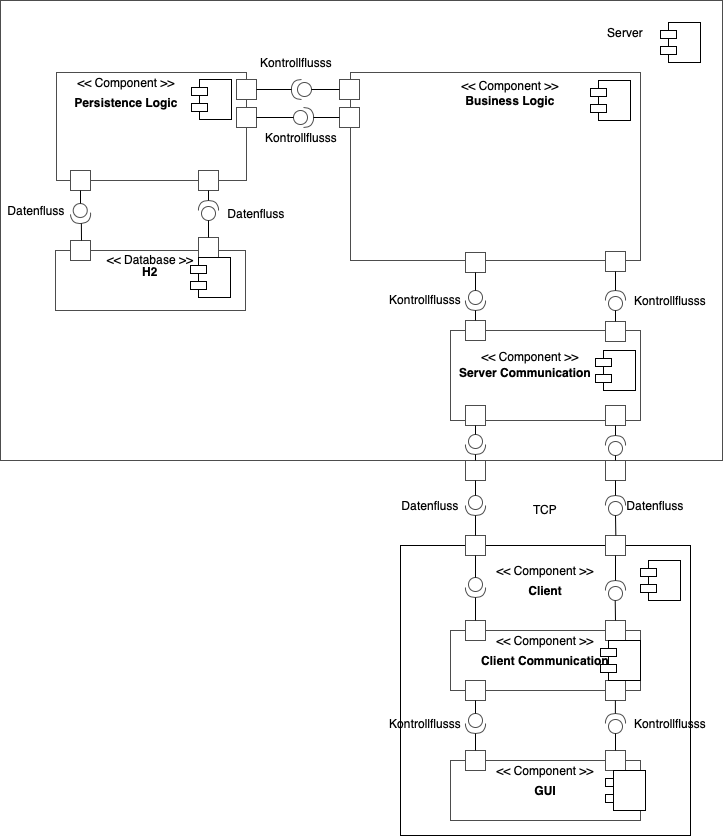
\includegraphics[width=0.85\textwidth]{Konzeptionelle_Sicht.png}
	\caption{Konzeptionelle Sicht}
	\label{fig1}
\end{figure}

{\itshape Diese Sicht beschreibt das System auf einer hohen Abstraktionsebene,
d.\,h. mit sehr starkem Bezug zur Anwendungsdomäne und den geforderten
Produktfunktionen und "~attributen. Sie legt die Grobstruktur fest, ohne gleich 
in die Details von spezifischen Technologien abzugleiten. Sie wird in den 
nachfolgenden Sichten konkretisiert und verfeinert. Die konzeptionelle Sicht 
wird mit {UML}-Komponentendiagrammen visualisiert.}


%%%%%%%%%%%%%%%%%%%%%%%%%%%%%%%%%%%%%%%%%%%%%%%%%%%%%%%%%%%%%%%%%%%%%%%%
\section{Modulsicht} \label{sec:modulsicht}

{\itshape Diese Sicht beschreibt den statischen Aufbau des Systems mit Hilfe von
Modulen, Subsystemen, Schichten und Schnittstellen. Diese Sicht ist 
hierarchisch, d.\,h. Module werden in Teilmodule zerlegt. Die Zerlegung endet 
bei Modulen, die ein klar umrissenes Arbeitspaket für eine Person darstellen und
in einer Kalenderwoche implementiert werden können. Die Modulbeschreibung der 
Blätter dieser Hierarchie muss genau genug und ausreichend sein, um das Modul 
implementieren zu können.

Die Modulsicht wird durch {UML}-Paket- und Klassendiagramme visualisiert.

Die Module werden durch ihre Schnittstellen beschrieben.
Die Schnittstelle eines Moduls $M$ ist die Menge aller Annahmen, die andere 
Module über $M$ machen dürfen, bzw.\ jene Annahmen, die $M$ über seine 
verwendeten Module macht (bzw. seine Umgebung, wozu auch Speicher, Laufzeit 
etc.\ gehören).
Konkrete Implementierungen dieser Schnittstellen sind das Geheimnis des Moduls
und können vom Programmierer festgelegt werden. Sie sollen hier dementsprechend 
nicht beschrieben werden. 

Die Diagramme der Modulsicht sollten die zur Schnittstelle gehörenden Methoden
enthalten. Die Beschreibung der einzelnen Methoden (im Sinne der 
Schnittstellenbeschreibung) geschieht allerdings per Javadoc im zugehörigen 
Quelltext. Das bedeutet, dass Ihr für alle Eure Module Klassen, Interfaces und 
Pakete erstellt und sie mit den Methoden der Schnittstellen verseht. Natürlich 
noch ohne Methodenrümpfe bzw.\ mit minimalen Rümpfen. Dieses Vorgehen 
vereinfacht den Schnittstellenentwurf und stellt Konsistenz sicher.

Jeder Schnittstelle liegt ein Protokoll zugrunde. Das Protokoll beschreibt die 
Vor- und Nachbedingungen der Schnittstellenelemente. Dazu gehören die erlaubten
Reihenfolgen, in denen Methoden der Schnittstelle aufgerufen werden dürfen, 
sowie Annahmen über Eingabeparameter und Zusicherungen über Ausgabeparameter. 
Das Protokoll von Modulen wird in der Modulsicht beschrieben.
Dort, wo es sinnvoll ist, sollte es mit Hilfe von Zustands- oder 
Sequenz-diagrammen spezifiziert werden. Diese sind dann einzusetzen, wenn der
Text allein kein ausreichendes Verständnis vermittelt (insbesondere bei 
komplexen oder nicht offensichtlichen Zusammenhängen).

Der Bezug zur konzeptionellen Sicht muss klar ersichtlich sein. Im Zweifel 
sollte er explizit erklärt werden. Auch für diese Sicht muss die Entstehung 
anhand der Strategien erläutert werden.}


%%%%%%%%%%%%%%%%%%%%%%%%%%%%%%%%%%%%%%%%%%%%%%%%%%%%%%%%%%%%%%%%%%%%%%%%
\section{Datensicht} \label{sec:datensicht}

{\itshape Hier wird das der Anwendung zugrundeliegende Datenmodell beschrieben. 
Hierzu werden neben einem erläuternden Text auch ein oder mehrere 
{UML}-Klassendiagramme verwendet. Das hier beschriebene Datenmodell wird u.\,a.\ 
jenes der Anforderungsspezifikation enthalten, allerdings mit 
implementierungsspezifischen Änderungen und Erweiterungen. Siehe die gesonderten
Hinweise.}


%%%%%%%%%%%%%%%%%%%%%%%%%%%%%%%%%%%%%%%%%%%%%%%%%%%%%%%%%%%%%%%%%%%%%%%%
\section{Ausführungssicht} \label{sec:ausfuehrung}

{\itshape Die Ausführungssicht beschreibt das Laufzeitverhalten. Hier werden die
Laufzeitelemente aufgeführt und beschrieben, welche Module sie zur Ausführung 
bringen. Ein Modul kann von mehreren Laufzeitelementen zur Laufzeit verwendet 
werden. Die Ausführungssicht beschreibt darüber hinaus, welche Laufzeitelemente 
spezifisch miteinander kommunizieren. Zudem wird bei verteilten Systemen 
(z.\,B.\ Client-Server-Systeme) dargestellt, welche Module von welchen Prozessen
auf welchen Rechnern ausgeführt werden.}


%%%%%%%%%%%%%%%%%%%%%%%%%%%%%%%%%%%%%%%%%%%%%%%%%%%%%%%%%%%%%%%%%%%%%%%%
\section{Zusammenhänge zwischen Anwendungsfällen und Architektur}
\sectionmark{Zusammenhänge AF u. Architektur} \label{sec:anwendungsfaelle}

{\itshape In diesem Abschnitt sollen Sequenzdiagramme mit Beschreibung(!) für 
\variante{zwei bis drei von Euch ausgewählte Anwendungsfälle}%
{einen von Euch ausgewählten Anwendungsfall}
erstellt werden. Ein Sequenzdiagramm beschreibt den Nachrichtenverkehr zwischen 
allen Modulen, die an der Realisierung des Anwendungsfalles beteiligt sind. 
\variante{Wählt die Anwendungsfälle so, dass nach Möglichkeit alle Module Eures
entworfenen Systems in mindestens einem Sequenzdiagramm vorkommen. Falls Euch 
das nicht gelingt, versucht möglichst viele und die wichtigsten Module 
abzudecken.}%
{Dazu könnt ihr Euch einen Anwendungsfall heraussuchen, der möglichst viele 
Module der  Architektur abdeckt. In SWP-2 werden wir mehrere Anwendungsfälle
betrachten und eine umfangreichere Abdeckung der Architektur anstreben.} }


%%%%%%%%%%%%%%%%%%%%%%%%%%%%%%%%%%%%%%%%%%%%%%%%%%%%%%%%%%%%%%%%%%%%%%%%
\section{Evolution} \label{sec:evolution}

{\itshape Beschreibt in diesem Abschnitt, welche Änderungen Ihr vornehmen müsst,
wenn sich Anforderungen oder Rahmenbedingungen ändern. Insbesondere würden 
hierbei die in der Anforderungsspezifikation unter \glqq{}Ausblick\grqq{} 
genannten Punkte behandelt werden.}

\dots

\end{document}

%%% Local Variables: 
%%% mode: latex
%%% mode: reftex
%%% mode: flyspell
%%% ispell-local-dictionary: "de_DE"
%%% TeX-master: t
%%% End: 
